This section is based on information from the book AI techniques for game programming\cite{buckland2002ai} chapter 7, 8 \& 9. Also from the book Neural networks: a systematic introduction\cite{rojas1996neural} chapter 7.
\\[0.5cm]
Neural networks are models that imitate the brains behaviour. They have been created as an option to model artificial intelligence and analyse machine learning. The human brain is made up of billions of neurons that are interconnected in a big grid. They communicate by firing electrical shocks through the network of neurons. The human brain is extremely complex and can calculate vast amounts of data in no time. This is why scientist and mathematicians have been trying to emulate this behaviour to create artificial intelligence.

\begin{figure}[weight!]
\centering
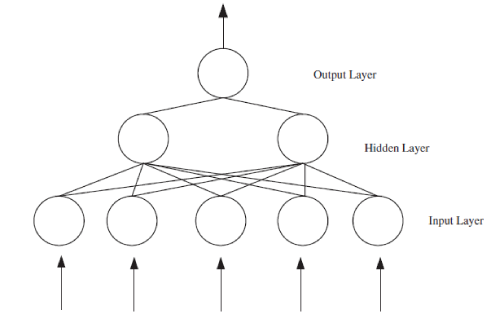
\includegraphics[width=0.8\linewidth,natwidth=898,natheight=587]{billeder/ANN.png}
\caption{A simple neural network with 3 layers. \cite{stockForecasting}}
\label{fig:weight_of_layers}
\end{figure}

Artificial neural networks (ANN) are artificial neurons (nodes) that are connected in a network. The network consists of an arbitrary number of layers that are interconnected. The most common structures in these networks are a feed forward structure. This kind of structure has the characteristic that it only flows data from the input layer through the layers to the output layer. There are no loops in the network thus making it unable to reiterate any information. Normally all of the nodes in the input layer is connected to all of the nodes in the second layer. The same connections are done in the next layers until we hit the output layer. This will give us he sum of all the previous nodes(\begin{math}x_i\end{math}) and their weights(\begin{math}w_i\end{math})(\begin{math}\sum_{i=0}^{i=n+1} w_i x_i \end{math}) in every node in the next layer:
\begin{figure}[weight!]
\centering
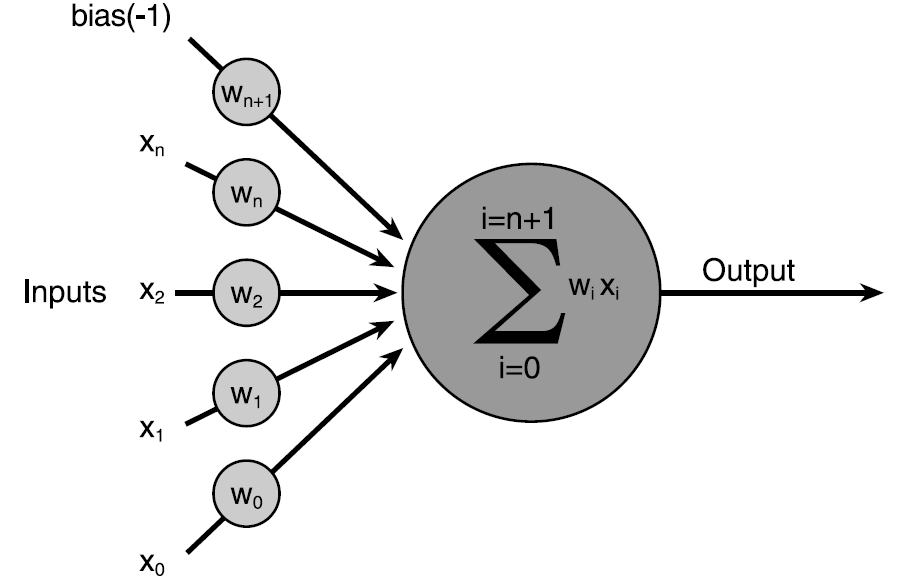
\includegraphics[width=0.8\linewidth,natwidth=898,natheight=587]{billeder/weight_of_layers.png}
\caption{How the weight is calculated from one layer to the next}
\label{fig:weight_of_layers}
\end{figure}
All of these connections carry a weight that dictates how data flows through the network and reflects the relations between the inputs and the outputs of the network. The inputs of the network should be all the factors that has an influence on the output we want from the network. In our example we would want to input; weather data, temperature, demand, availability \cite{21} to get the price as an output from the network.

Every node in our network contains an activation function. This function, when calculated, tells us whether the artificial neuron should fire or not. That is, if the neuron should transmit the data from the current layer to the next layer. There are a lot of different activation functions. The simplest form is the binary step function which either fires or it does not. This depends on the input and gives us a low threshold of complexity which is good in simple neural networks as the relations between the nodes do not need to be that fine grained. In more complex systems we want activation functions with a broader output range than binary. In many cases a sigmoid function is used as the activation function. This is because of the ''S''-shape which enables it to compute outputs in a non-linear way. The non-linear nature of the sigmoid functions is what makes the neural network able to compute non-trivial problems in reasonable sized networks. The sigmoid function allows the activation functions of the neurons to have a broader range of inputs which will produce an output compared to step activation functions. To be able to calculate a non-trivial problem in these kind of networks we need what is called a training algorithm. This algorithm depicts how the network evolves over time also known as learning. There are two kinds of learning; supervised learning and unsupervised learning.

\section{Unsupervised learning}
Unsupervised learning is when we do not have prior data to base our work on. Instead we have a problem where we want the neural network to try and estimate its behaviour relative to a specific task based on some assumptions we have about the system it performs on. It is commonly used with estimation problems like "Cluster Analysis", which in short is attempting to fit data into clusters of data that have some of the same criteria. This is often done by exploring the dataset and that is what unsupervised learning is good for. It also works with Artificial Intelligence(AI) that have to explore parts of the (virtual)world. In \cite{buckland2002ai} he explains how an unsupervised learning feed-forward artificial neural network trains itself using a genetic algorithm to keep track of the fitness function of the AI. The fitness function is used to tell the AI if it is doing good or doing bad and is used for training the network. It will get a plus score in the fitness function if it encounters what we are looking for and get negative if it hits something that we defined as "wrong". Based on this fitness function it will update the weights of the neural network accordingly to what is most beneficial for the network as a total. After it has been allowed to do a lot of runs it begins to get a sense of what it is exploring and should be able to make better choices for each run.

\section{Supervised learning}
Supervised learning are a set of algorithms that use a dataset which contains both the inputs and what the output is expected to be. This dataset is used to train the neural network to make it able to do calculations on data and predict the outcome. An example of an algorithm used for supervised learning is the backpropagation algorithm. 
It starts out by randomly assigning all the weights on the connections between the neurons. It then calculates the output of the network and compares it to the expected output. From that it calculates the error margin between the expected and the calculated output and adjusts the weights accordingly. This is done for all the hidden layers as well until we hit the input layer. All of these steps are called an epoch. We will repeat as many epochs as we need until the sum of all the errors are within a given threshold. The name of the algorithm originated from this approach where it propagates the error backwards in the network.

Supervised learning can be thought of as learning with a teacher. As an example we can use the XOR table:

\begin{table}[h!]
\centering  % used for centering table
\begin{tabular}{c c c} % centered columns (3 columns)
Input \#1 & Input \#2 & Output \\ [0.5ex] % inserts table 
%heading
\hline                  % inserts single horizontal line
0 & 0 & 0  \\ % inserting body of the table
1 & 0 & 1  \\
0 & 1 & 1  \\
1 & 1 & 0 \\ [1ex] % [1ex] adds vertical space
\hline %inserts single line
\end{tabular}
\caption{This training set is very simple yet it illustrates a training set for a supervised learning algorithm very well.} % title of Table
\label{table:xor-table} % is used to refer this table in the text
\end{table}

In this dataset we have both of the inputs and we are given the expected output. This gives the backpropagation algorithm a direction to follow when minimizing the error function of the network. We can do this because we get an output that we can compare to the expected output which allows us to predict the direction that the error correction should take to come closer to the answer. Also the sigmoid activation function helps us closing in on the target output since the sigmoid function always has a positive derivative which ensures that we will always have a direction to follow\cite[p. 153]{rojas1996neural}. This is because the derivative of the sigmoid function always will point us towards the global minima of the expected function. If we take a look at ~\ref{table:xor-table} we are given inputs and outputs. We take the input 1 and 0 we expect the output to be 1. The neural network will initialize weights and start to run the backpropagation. The backpropagation algorithm will compare the output it gets to the output we expected e.g. we may get an output of 0.5 (based on the random weight initialization) and this is compared to the expected output 1. Because of the sigmoid function we know what direction the weights should be corrected to come closer to the output of 1. This allows the backpropagtion algorithm to recalculate the weights and be sure that it is heading for the global minima of the error function thus heading for the right output.
%[FORKLAR MATEMATIKKEN EVT MED EKSEMPEL s. 332 i bogen]

In neural networks bias neurons are often added to the layers to help them learn patterns. The bias neurons are added to give the activation functions the ability to change its output even if x is zero. If we look at the graph in figure ~\ref{fig:activationFunctions} it uses the following activation function: \begin{math} \frac{1}{(1+e^{(-cx)})} \end{math} where c is the weight.

\begin{figure}[weight!]
\centering
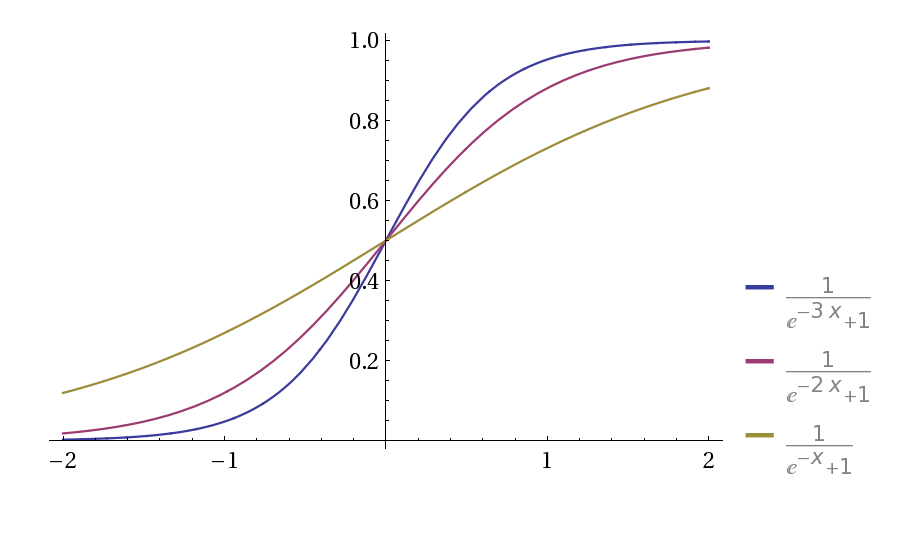
\includegraphics[width=0.8\textwidth ,natwidth=410,natheight=237]{billeder/ActivationFunctions.png}
\caption{}
\label{fig:activationFunctions}
\end{figure}

The figure shows how the gradient of the function alters with different weight values. Even though the gradient of the function is clearly altered by the weights the function is still outputting the same result for zero thus we cannot alter the output for x equal to zero just by altering the weights. This is what we use the bias for. If we apply a bias of one to all of the neurons we will be able to shift it either to the left or the right. In figure ~\ref{fig:activationFunctionsWithBias} we see the same function as before where the weight is set to 2. The difference is that we added a bias (b) to this function: \begin{math} \frac{1}{(1+e^{(-2x+b)})} \end{math} \cite[p. 165]{rojas1996neural} \cite{inductiveBias}

\begin{figure}[weight!]
\centering
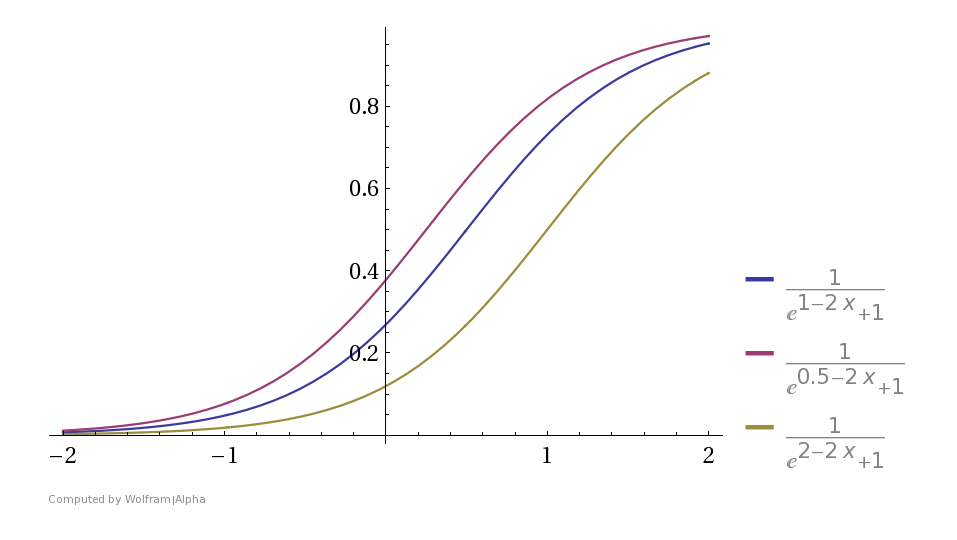
\includegraphics[width=0.8\textwidth ,natwidth=410,natheight=237]{billeder/ActivationFunctionsWithBias.png}
\caption{}
\label{fig:activationFunctionsWithBias}
\end{figure}

To calculate the error between input and output we use the mean squared error function. This function is given by: \begin{math} MSE=\frac{1}{n}\sum_{i=0}^{n}(\hat{y}_i-\bar{y}_i)^2 \end{math} where \begin{math} \hat{y}_i \end{math} is the ideal value and \begin{math} \bar{y}_i \end{math} is the actual value. We use this error calculation because it incorporates the bias \cite{meanSquaredError}

\section{Common pitfalls}
When we are trying to fit our algorithm and make it recognize patterns we will encounter several possible pitfalls. First of all there is the chance of ending up in a local minima. This is when the the backpropagation algorithm attempts to find the global minimum of the error curve, thus having reduce the error as much as possible. The algorithm works by trying to reduce this error margin a little step at a time. If it encounters a local minima on the curve and thinks it has reached the global minima it gets stuck and we will get inaccurate results. 

\begin{figure}
\centering
\begin{minipage}{.5\textwidth}
  \centering
  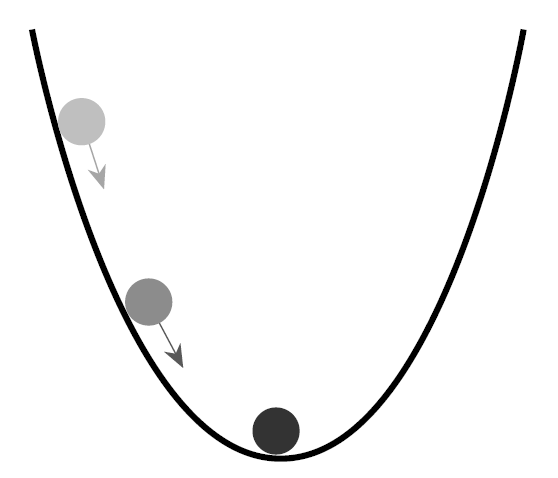
\includegraphics[width=.4\linewidth]{billeder/globalMinimum.png}
  \captionof{figure}{At the global minimum \cite[P. 318]{buckland2002ai}}
  \label{fig:test1}
\end{minipage}%
\begin{minipage}{.5\textwidth}
  \centering
  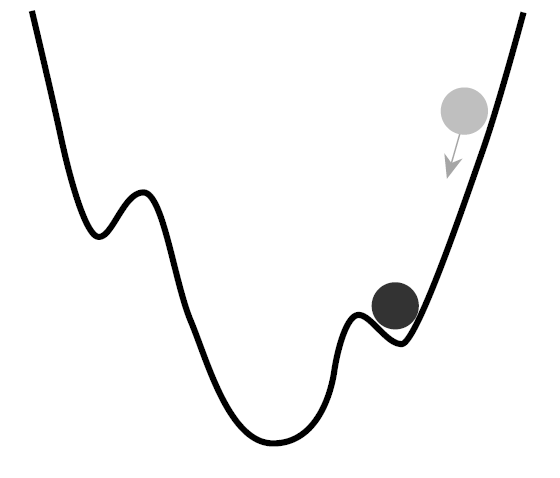
\includegraphics[width=.4\linewidth]{billeder/localMinimum.png}
  \captionof{figure}{Stuck in a local minimum \cite[P. 318]{buckland2002ai}}
  \label{fig:localMinimum}
\end{minipage}
\end{figure}

To avoid the backpropagation algorithm to falsely accept a local minima as the global minima we can give the algorithm momentum. This is done by adding a bit of the last error correction from the earlier layer to the next layers error correction. This way the algorithm, so to say, will scoot right by any small deviations in the error correction face.
\newline
Another pitfall when working with neural networks is over fitting the algorithm. This is when the algorithm instead of finding a generalized pattern in the inputs it will find an over-fit pattern that will fit exactly that input. This is better shown in figure ~\ref{fig:overfitting}.
\begin{figure}[h!]
\centering
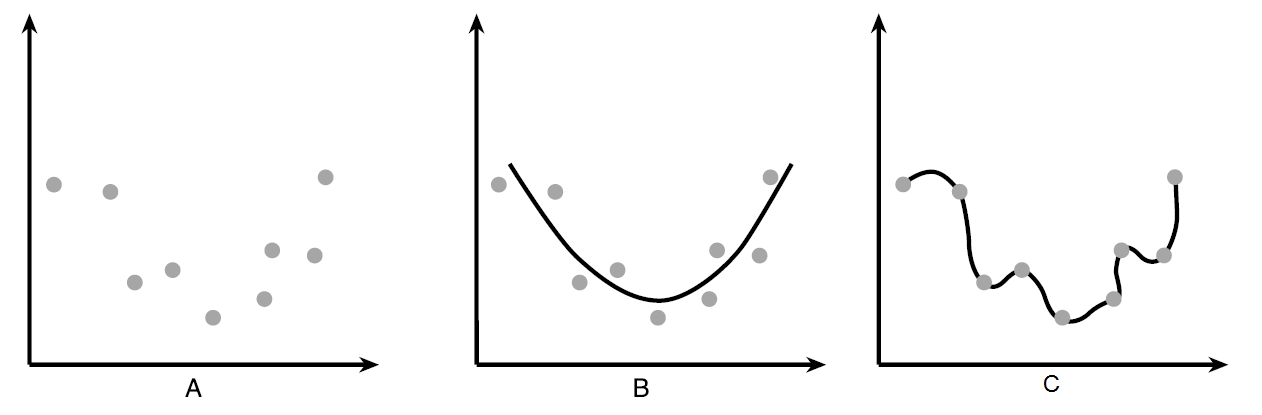
\includegraphics[width=0.8\linewidth,natwidth=1262,natheight=415]{billeder/overfitting.png}
\caption{A. The plot graph of the input B. The generalized function C. An over-fit function}
\label{fig:overfitting}
\end{figure}
This can be avoided by some simple techniques. First of all we want to reduced the neurons as much as possible as long as it does not interfere with our performance of the system. This is a trial and error problem and has to be tweaked along with evolving your neural network. We can add noise to avoid this problem. By adding noise(random data values) we prevent the algorithm from fitting the function to closely to the given data. Thus giving us a more generalized function where it hopefully will be able to fit new data presented to it better. Early stopping is another method to avoid over-fitting. This is only doable with large datasets where you can split it into two equal datasets. The first will work as a training set and the second will work as a validation set. We will keep training the dataset and checking with the validation set until the difference between those two start to increase.

